To achieve a self-consistent simulation, it is necessary to take the back-reaction into account by evolving the mass and acceleration along with the field itself. The long term goal is to perform an accurate study of the differences between the geodesic evolution method used in Niels Warburton's frequency domain technique and the self-consistent evolution method used in Peter Diener's time domain technique for the scalar approximation to the extreme mass ratio inspiral problem. Diener and Warburton have implemented a preliminary simulation that uses initial conditions from the geodesic case to as a consistency check of the low order modes in the self-consistent simulation. Our simulation has some stability issues that must be addressed to evolve for longer durations. One possible explanation is the truncation error. Another possibility is with the sum of the l-modes. A specific functional form is fit over intermediate values of l to extend the sum analytically past the highest l-mode computed to $l=\infty$. There are uncertainties associated with the manner in which this sum is performed. In this chapter, I explore the truncation error associated with the first order Richardson extrapolation.

\section{First order Richardson extrapolation}

The Discontinuous Galerkin method results in truncation error that scales as $h^{N+1}$, where $h$ is the element size and $N$ is the order of the interpolating polynomials within the element.~\cite{dghesthaven} The radial self force is given by the radial derivative of the scalar field, $F_r=\partial_r\Psi$. However, to obtain this quantity, it is necessary to sum the radial derivatives over all $l$ and $m$ modes. Let $F_l=\sum_{m=-l}^l F_{lm}$. Each of these modes, separately, follows the DG convergence scaling laws. It should be possible to extrapolate to infinite DG order based and obtain the first order Richardson extrapolation, $F_{inf}$, which is the self force for a given l-mode at infinite DG order after a single iteration of the extrapolation of the errors. If the Richardson extrapolation were extended to second order, the error of the error may take on a different functional form, and the second order extrapolation may require a different technique; however, I do not perform it because there is too much random noise in the second order error to determine a functional form.

The three-point exponential extrapolation is motivated by our assumption that Discontinuous Galerkin error is one-sided in the truncation error regime-- it is not random; hence, the self force more or less monotonically approaches a limit. In the round-off error regime where the error is random, the self-force is no longer monotonically converging. As long as it is monotonically converging, it can be written in the form of $F_r(n,l)=F_{inf}(l)+c(l)\exp[-\alpha n]$, where $n$ is the DG order. For a given mode, there is a four step procedure for determining the three parameters associated with the Richardson extrapolation. A root finding technique must be used to solve the following system of equations to determine the exponent of the self force. $\alpha$ must be greater than zero, since the self force is converging with DG order. We use the bisection method. 
\begin{eqnarray}
g(\alpha)-P=&0\\
g(\alpha)=&\frac{\exp[\alpha(n_1-n_2)]-1}{-1+\exp[\alpha(n_1-n_3)]}\\
P=&\frac{F_r(n_1,l)-F_r(n_2,l)}{F_r(n_1,l)-F_r(n_3,l)}
\end{eqnarray}
Secondly, the mode-dependent coefficients of the exponent must be determined.
\begin{equation}
c(l)=\frac{F_r(n_1)-F_r(n_2)}{\exp[-\alpha n_1]-\exp[-\alpha n_2]}
\end{equation}
Finally, the first order Richardson extrapolation, the value of the self force at infinite order, to first order in the errors, depends on the l-mode and the time. The time dependence is implicit in the time dependence of $F_r(n_3)$. 
\begin{equation}
F_{inf}(l,t)=F_r(n_3)-c(l)\exp[-\alpha n_3]
\end{equation}

Sometimes there is not a solution due to roundoff noise causing a deviation from the expected exponential behavior. In practice we allow all three parameters to vary with l-mode and time. I use extrapolation starting orders from the set 12, 16, 20, 24, 28, 32, and 36, with additional data at orders 40 and 44 that may be used as points two and three. Sets of three consecutive DG orders on this list were used. In order to use data from several different DG orders, it was necessary to interpolate between the times at which each order was computed to some desired common set of times. Each order uses different time steps for Courant stability, which requires that time steps are less than the wave travel time to the minimum spacing on the grid. Interpolation was performed using a cubic polynomial scheme. 


\section{Choice of starting order}

Some modes fail because roundoff noise causes the data to deviate from exponential convergence, it is not possible to chose the same starting order for the extrapolation for all modes and all times. This can be done manually, but to produce an evolution over the entire time series to investigate the error as a function of time, it is desirable to automate this process.

\subsection{The last non-NaN method}

The first attempt I made to improve the choice of starting order was to chose the highest starting order for which no lower starting order had been unsolvable. Figure~\ref{finfovertimediscont} shows this approach leads to some discontinuities in the time evolution of $F_{inf}$ in some l-modes ($l=3$ is shown). 


\begin{figure}
  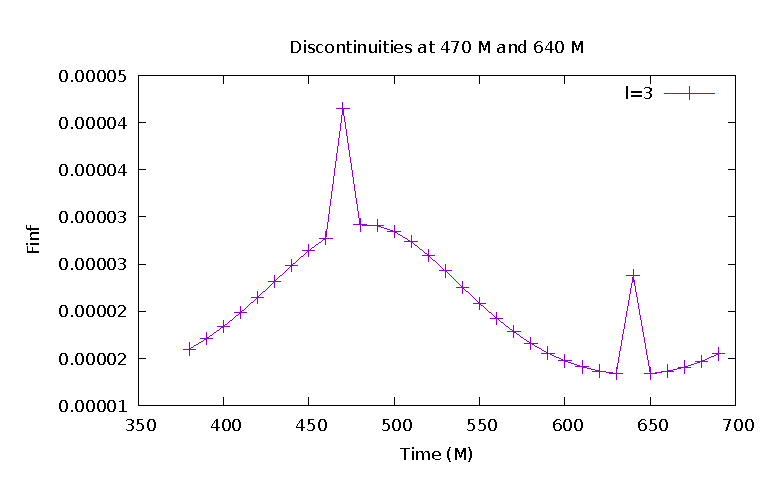
\includegraphics{finfovertimel3discontinuities}
  \caption{Starting order was chosen by iterating from the lowest order to the first order for which the starting order had no solution, and choosing the maximum starting order that succeeded. When $F_{inf}$ is evolved over one full orbital cycle, some l-modes shows discontinuities at some times. l=3}
\label{finfovertimediscont}
\end{figure}

\subsubsection{Manually correcting badly selected automatic values}
To address this concern, I examined the choice of starting order more closely for specific times where discontinuities were present. If the DG orders converged perfectly, they would form a line in semi-log space once $F_{inf}$ is subtracted, if it could be subtracted perfectly. See Figure~\ref{goodbehavior} for an example. Some less perfect examples are shown below. This time is particularly bad, which is why it produced the glitch that requires investigation. $l=2$ and $t=632M$, is shown in a Table~\ref{manual}. Figure~\ref{nosoln} shows an example where no solution is found. The roundoff noise is visible in Figure~\ref{roundoff} at high DG orders. In Figure~\ref{offset}, it is possible the effect at high DG orders is roundoff noise in the $F_r(n,l)$ values of the points, but it is more likely that it is roundoff noise in the choice of $F_{inf}$ due to limitations of the root finding method, resulting in an incorrect offset of the curve. Figure~\ref{manualfix} shows that after selecting an average of the reasonably similar values from Table~\ref{manual}, the discontinuity in the $l=2$ $t=632M$ radial self-force becomes smooth. 


\begin{table}
  \begin{tabular}{ll}
    Starting Order & $F_{inf}$\\
    12 & no solution\\
    16 & 2.40975299617e-05\\
    20 & 2.40975300465e-05\\
    24 & 2.40975300114e-05\\
    28 & no solution\\
    32 & 2.40975299291e-05\\
    36 & 2.40975299148e-05\\
  \end{tabular}
  \caption{Manual starting indices and $F_{inf}$ values for t=632, l=2.}
  \label{manual}
\end{table}

\begin{figure}
  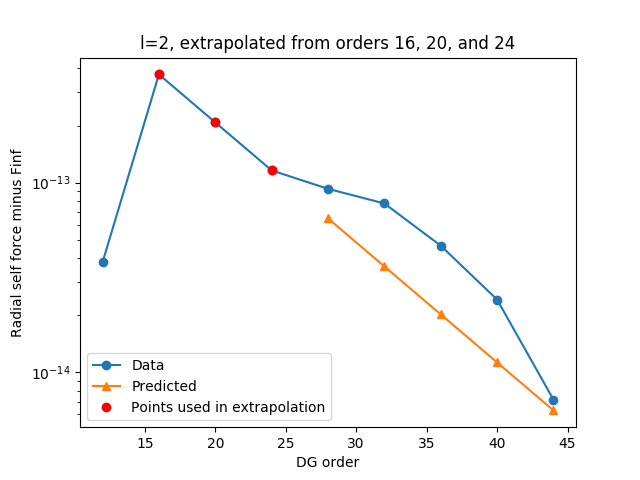
\includegraphics{extrapolate7t632l2i1}
  \caption{Radial self-force with $F_{inf}$ subtracted. Fluctuation in one of the points chosen in the extrapolation, due to roundoff or truncation error, causes the extrapolation to predict a value of $F_{inf}$ that is subtly wrong, leading to curvature in the semi-log plot after $F_{inf}$ subtraction. t=632, l=2, starting order 16}
  \label{nosoln}
\end{figure}

\begin{figure}
  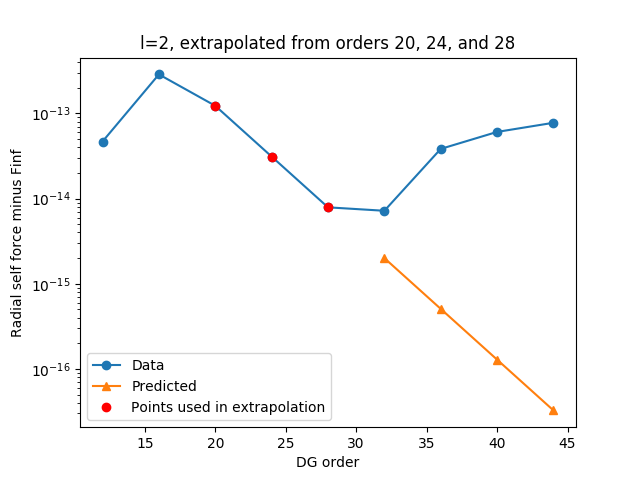
\includegraphics{extrapolate7t632l2i2}
  \caption{Roundoff error is visible at high DG orders. t=632, l=2, i=2}
  \label{roundoff}
\end{figure}

\begin{figure}
  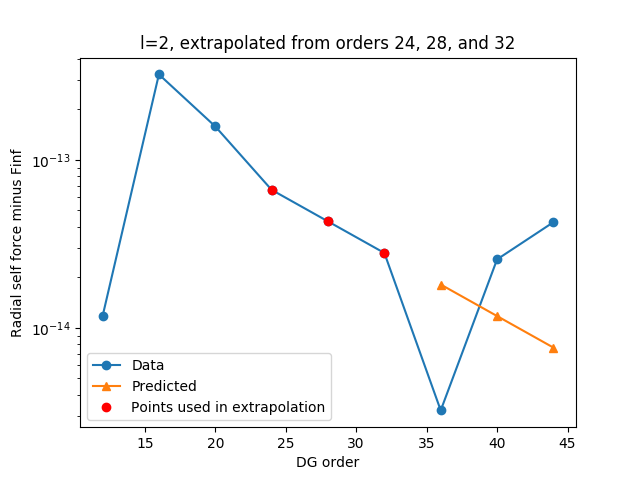
\includegraphics{extrapolate7t632l2i3}
  \caption{Radial self-force with $F_{inf}$ subtracted. The incorrect value of $F_{inf}$ has been chosen due to roundoff error, perhaps due to finite precision in the root finding algorithm, leading to a negative values, that show as a ``V'' in the semi-log plot. t=632, l=2, starting order 24}
  \label{offset}
\end{figure}


\begin{figure}
  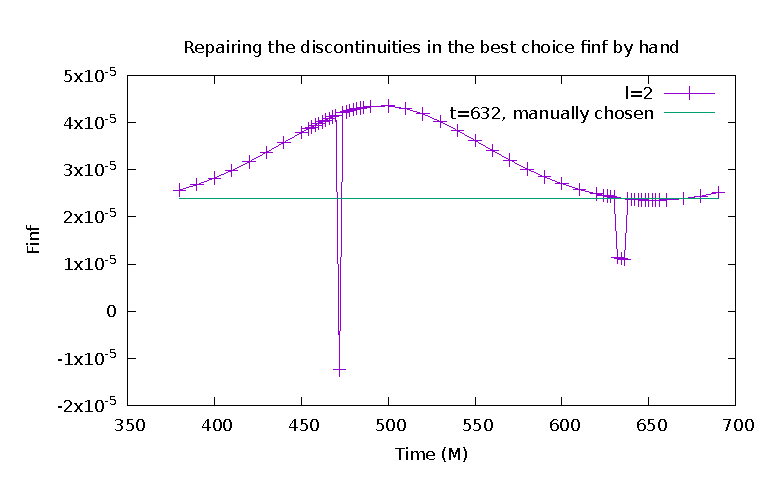
\includegraphics{bestFinfManuallyChosent632l2}
\caption{$F_{inf}$ as a function of time. Manual correction for discontinuities in the l=2 mode, using the manually determined $F_{inf}$ data from Table~\ref{manual}. }
\label{manualfix}          
\end{figure}

\subsection{The median method}

To resolve the discontinuity problem, I attempted another approach. I ordered the starting orders that had a solution at each time and for each mode by their $F_{inf}$ values. The median value of $F_{inf}$ was selected, in the hope that it will discard those effected by roundoff and those effected by failure to converge. However, there is no guarantee that it selects those in this regime, since in principle a mode could both be in the roundoff limit and have not converged yet. Yet when this is done, there are no discontinuities in $F_{inf}$ for any of the l-modes when the median approach is used. See mode zero for an example..

\begin{figure}
  \includegraphics{finfovertimel0}
  \caption{An example of no discontinuities in $F_{inf}$ for any of the l-modes. Mode $l=0$.}
\end{figure}


\subsection{The fit method}
A better motivated approach, is to fit subsegments of lines in semi-log space on the DG order convergence plot, and find the longest and most linear region. A fit with the ``best'' value of the reduced chi squared should be a good approximation to this. The reduced chi squared is the value of the sum of the residuals of the fit squared divided by the number of degrees of freedom, which in this case is the number of points in the fit minus two, since there are two degrees of freedom in a linear fit. The expectation value of the reduced chi squared, in the limit of a large number of degrees of freedom, is one. I loop over starting and ending points of the fit, and over starting orders, and choose the starting order with the best fit line segment in the sense that that line segment has a reduced chi squared closest to one. An example of such an automatically chosen starting index is given in Figure~\ref{autoconverge}, where there is a long exponentially converging region. Figure~\ref{abserrfitmedian} shows that the absolute error between fit and median techniques increases with l-mode, possibly indicating that roundoff error becomes a more significant factor in the median technique as the l-mode increases, and the fit technique becomes more important. 

\begin{figure}
  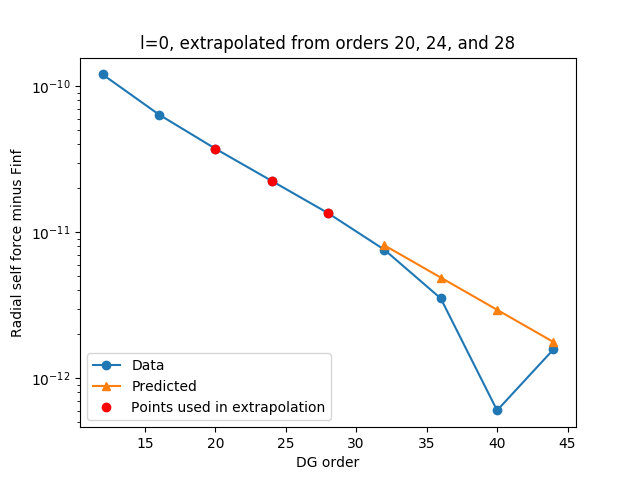
\includegraphics{fittingtechniqet370l0}
  \caption{l=0 mode with line-segment fit-chosen starting order produces convergence plot with long exponentially converging region}
  \label{goodbehavior}
\end{figure}

The absolute error between the fit and median methods increases with l-mode suggesting that roundoff error becomes more important at higher l-modes.

\begin{figure}
  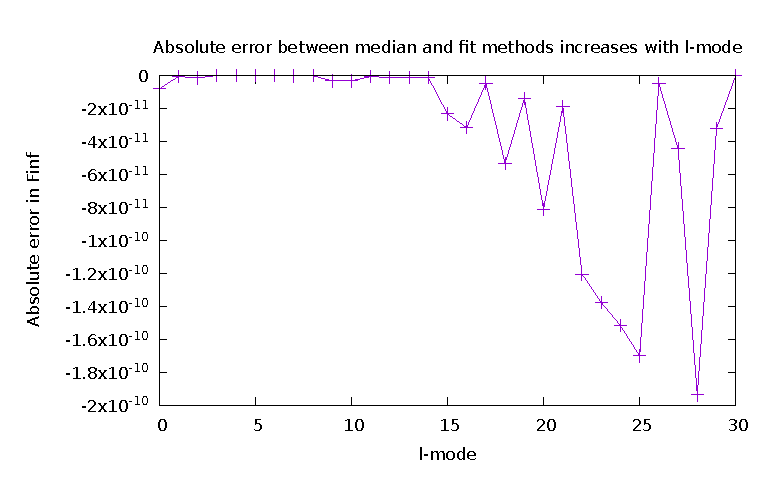
\includegraphics{absErrorIncreaseslmode}
  \caption{Absolute error between fit and median techniques increases with l-mode.}
\end{figure}

There are some outstanding issues with this method. Specifically, I am concerned about the normalization of the the reduced chi-squared, given the unspecified normalization of the second order errors; however, this doesn't seem to prevent the algorithm from nearly working, so perhaps the normalization is nearly correct by chance. Secondly, the fact that the three points used in the extrapolation on the self-force minus $F_{inf}$ curve are precisely on a line in semi-log space means that any hypothesis test is going to be skewed to preferentially select regions including only those three values. To correct for this, it might be better to consider a statistic based upon residuals to the parameters obtained by the extrapolation, with the number of degrees of freedom adjusted to account for the three fixed points. The second order noise is plainly not Gaussian or even unbiasedly distributed, so it is not simple to calculate an expectation value for such a statistic; however, it should have properties similar to the reduced chi squared, so in a back-of-the-envelope sense, can probably be compared to that statistic with the appropriate choice of the degrees of freedom. The biased nature of the second order truncation error is also an issue when using the chi squared test in its usual form. 



\section{The asymptote method}

In a third approach, I consider the behavior of $F_{inf}$ as a function of starting order of the extrapolation. In many, but not all, modes, $F_{inf}$ appears to converge to an asymptote from above or below as the DG starting order increases. However, in many modes, some starting orders produce no solution, so our set of six DG starting orders is reduced to somewhere between three and five. There are two obvious ways to test for convergence: fit an exponent or a power law and do a likelihood ratio test relative to a constant (since the second order errors are unmodelled), or, more reasonably, examine the signs of the first and second numerical derivatives with respect to DG order and consider the end of the convergent regime to be the point where the roundoff noise dominates, and the product of the sign of the derivatives becomes positive. From this derivative sign test, we can determine the best starting order for $F_{inf}$ of a pattern of five or six points that are behaving in a converging like pattern.

However, sometimes, due to high roundoff noise or non-convergent behavior, a low DG order is chosen even for the case where there are five or six good contiguous starting indices. In that case, the asymptotic value of $F_{inf}$ at high DG orders is under-estimated. To achieve a better estimate, I sort this group into the same class as the two, three, and four length contiguous sets of successful DG orders that generated values of $F_{inf}$. For this case, I make an assumption that except for one or maybe two outliers, $F_{inf}$ is approximately constant across the range. The outliers may be at the beginning or the end, or may be due to roundoff noise fluctuations. To reject outliers, I do a standard statistical test of taking the average, making a veto based on the number of standard deviations a point is away from the average, and taking an average again using only the data that survived the veto. I select the point with the value closest to the second average as the best starting order for the extrapolation, and the value I will use to obtain $F_{inf}$. In this case, I found that I got linear curves of $\Psi_r-F_{inf}$ on a semi-log scale for a one sigma veto.

After performing this selection of the best starting order, based on methods to look for asymptotes or reject outliers, I obtained the time evolution of the radial self force, summed from $l=0$ to $l=30$, shown in Figure~\ref{summixed}. The absolute error between $F_{inf}$ and the different DG orders is shown in Figure~\ref{absmixed} and the relative error is shown in Figure~\ref{relmixed}. There is one time where there is some kind of glitch in $F_{inf}$ that remains to be investigated; however, the evolution as a whole appears to be smooth. The absolute and relative error demonstrate that convergence is exponential until about DG order 36 or 40, and which point roundoff noise takes over. The best order for evolutions is therefore DG order 36. The spike is due to $l=25$ at $t=630$, where there is no starting order for which a solution exists. We have examined the time series data and there appears to be some truncation error in mode 16. There also appears to be some roundoff error in $l=25$ at $t=630$, though I have not yet compared it to other times. The truncation error in $l=16$ does not explain the lack of solutions in the extrapolations starting from higher DG orders. The roundoff noise might provide an explanation for this problem, but needs further investigation. In particular, since in the next chapter I conclude that the maximum l-mode that should be included in the fit is $l=24$, I intend to try summing to $l=24$ instead (though this will take significantly more work to implement). The error due to our inability to use a Richardson extrapolation in real time is at the level of $10^{-4}$.

\begin{figure}
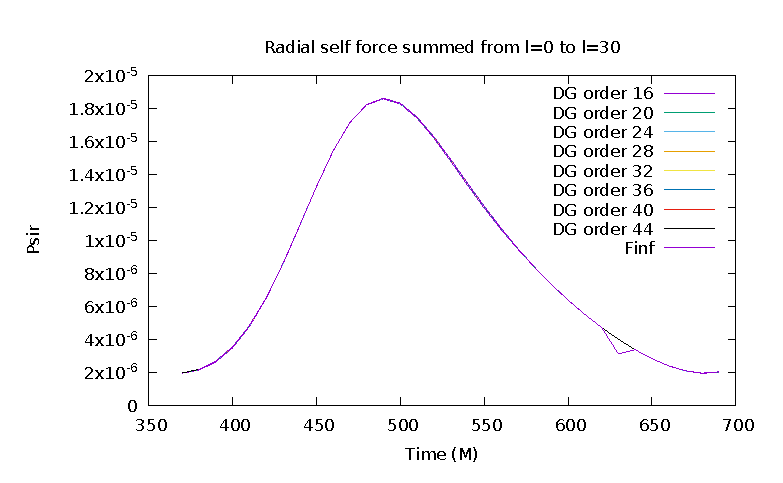
\includegraphics{psirvtwfinfdgorders}
\caption{Sum from $l=0$ to $l=30$ of the radial self force, comparing all DG orders to $F_{inf}$. This was obtained using the method based on asymptotes and averages with rejection of outliers.}
\label{summixed}
\end{figure}

\begin{figure}
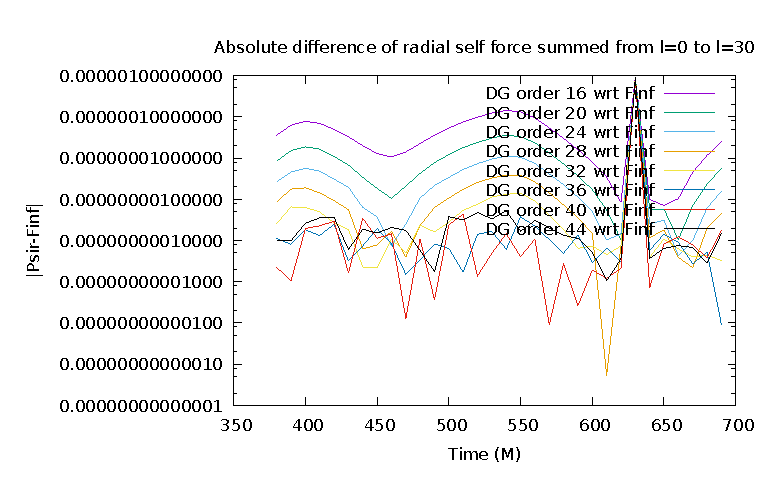
\includegraphics{absdiffpsirvtwfinfdgorders}
\caption{Absolute difference of the radial self force summed from $l=0$ to $l=30$  for each DG order compared to the total radial self force for these modes for $F_{inf}$. This was obtained using the method based on asymptotes and averages with rejection of outliers.}
\label{absmixed}
\end{figure}

\begin{figure}
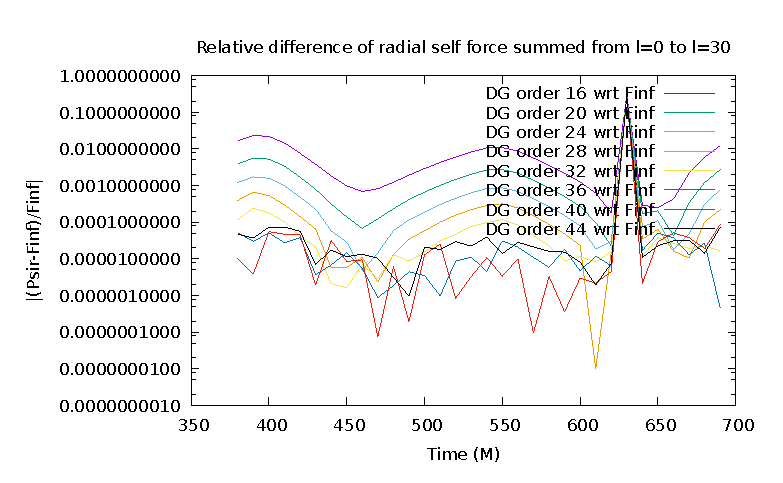
\includegraphics{reldiffpsirvtwfinfdgorders}
\caption{Relative difference of the radial self force summed from $l=0$ to $l=30$  for each DG order compared to the total radial self force for these modes for $F_{inf}$. This was obtained using the method based on asymptotes and averages with rejection of outliers. The error is at the $10^-4$ level.}
\label{relmixed}
\end{figure}
